\subsection{The Purpose of Neural Networks for Image Processing}

The purpose of utilizing neural networks in image processing is to algorithmically emulate the visual perception system found in animals (\cref{fig:nn-purpose-zebra}), specifically creating computational analogies to the physical neuronal pathways involved in visual processing.
It is often taken for granted that the human brain seamlessly interprets images regardless of orientation and extrapolates information from visual data. However, algorithmically replicating such innate capabilities has posed substantial challenges.
A key benefit of neural networks is the minimization of manual feature selection, which has traditionally constrained image processing methods.
By automating feature selection, neural networks can not only simplify image analysis procedures, but also enhance the capacity of these systems to computationally process and interpret images akin to the capabilities of the human brain.
Thus, neural networks represent an important advancement for the field of image processing.


\begin{figure}[h!]
  \centering
  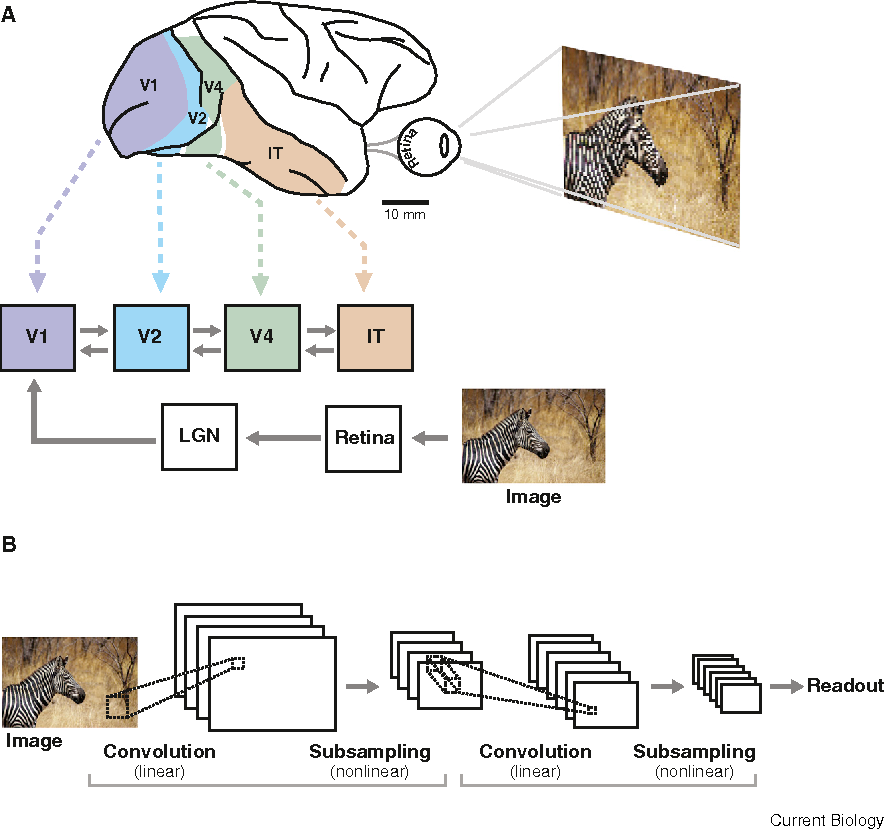
\includegraphics[width = 0.75\linewidth]{figures/raster/visual-nn.png}
  \caption{An example of a neural network mimicking the human brain.}
  \label{fig:nn-purpose-zebra}
\end{figure}

%%% Local Variables:
%%% mode: latex
%%% TeX-master: "../../../Andrew_Jensen_Dissertation"
%%% End:
